\documentclass{article}
\usepackage[utf8]{inputenc}
\usepackage{graphicx}
\usepackage{float}
\usepackage[a4paper,
            left=1in,
            right=1in,
            top=0.5in,
            bottom=1in,]{geometry}



\title{Autocorrelation in Florida Weather}
\author{Kayleigh Greenwood}
\date{November 2021}

\begin{document}

\maketitle

\section{Results}
The Kendall rank correlation coefficient was used to determine whether there was a positive correlation between Temperature in Key West, Florida, and the Temperature the following year. The correlation coefficient of the Temperature data throughout the years in the 20th century was 0.238342, and a permutation analysis (Figure 1) of 1000 shuffled populations was used to determine the approximate, asymptotic, one-tailed P-value of 0.

\begin{figure}[H]
\centering
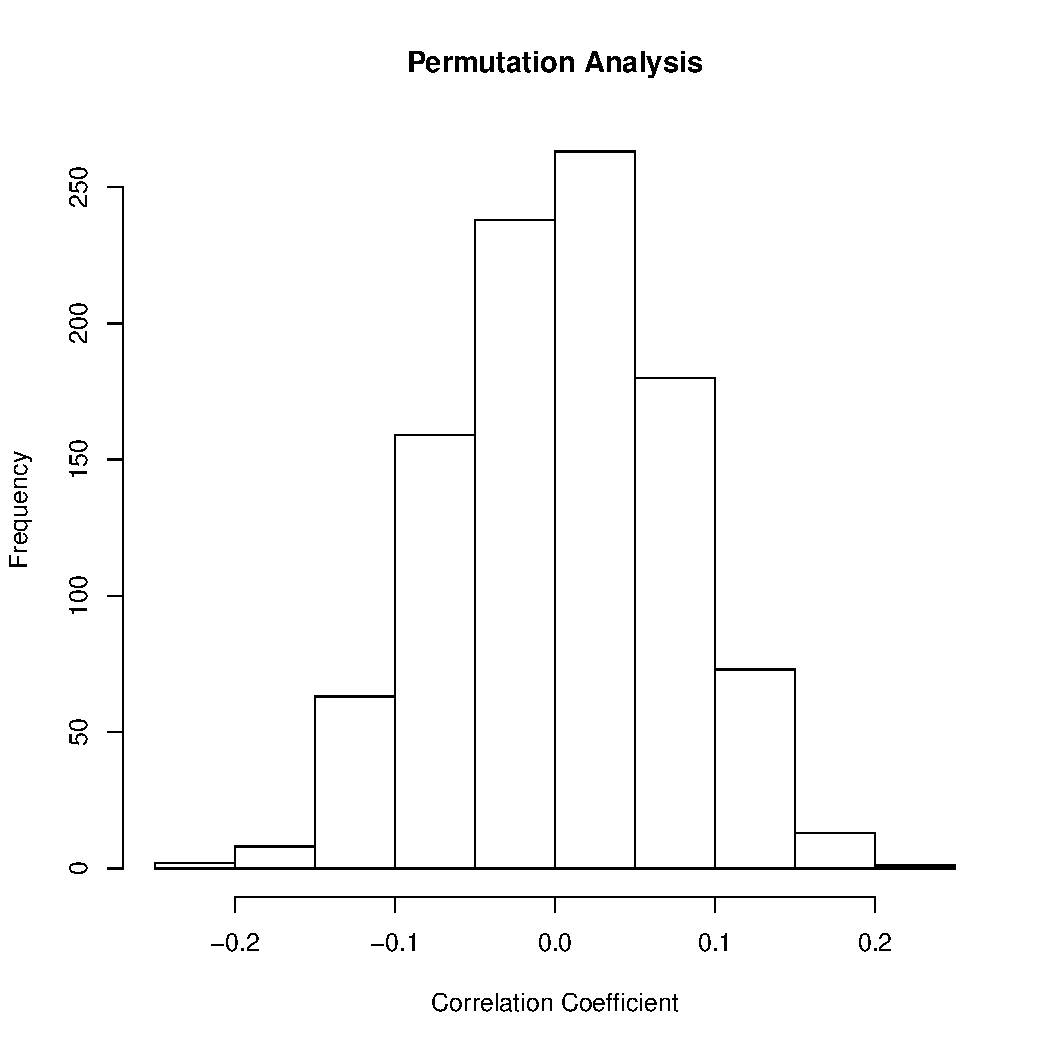
\includegraphics[scale=0.75]{../results/TAutoCorrhist.pdf}
\caption{Histogram of Coefficients}
\end{figure}

\section{Discussion}
 Given that the P-value was below 0.05, we can reject the null hypothesis that Temperature in Key West, Florida are not significantly correlated with the next year, and determine that there is a statistically significant positive correlation between the two variables. The positive correlation indicated between Temperature in Key West and Temperature the successive year is statistically significant.
These results suggest that throughout the 20th century, temperature was increasing over time in Key West.

\end{document}
